\documentclass[a4paper,11pt]{article}

\usepackage{exptech}       % Fichier (./exptech.sty) contenant les styles pour 
                           % l'expose technique (ne pas le modifier)
\usepackage{array}
%\linespread{1,6}          % Pour une version destinée à un relecteur,
                           % décommenter cette commande (double interligne) 
                           
% UTILISEZ SPELL (correcteur orthographique) à accès simplifi? depuis XEmacs

%%%%%%%%%%%%%%%%%%%%%%%%%%%%%%%%%%%%%%%%%%%%%%%%%%%%%%%%%%%%%%%%%%%%%%%%%%%%%%%
\begin{document}  

\begin{titlepage}
\begin{minipage}[t]{0.5\textwidth}
\begin{flushleft}
\centering
\hspace{-5cm}

\includegraphics[width=\textwidth]{fig/logoINSA}
\end{flushleft}
\end{minipage}
\begin{minipage}[t]{0.5\textwidth}
\begin{flushright}
\centering

\includegraphics[width=\textwidth]{fig/logo}
\end{flushright}
\end{minipage}
\vspace{8cm}
\begin{center}
\textsc{\LARGE \bfseries People Warfare}\\[0.25cm]
		{\LARGE Rapport de conception}\\[0.25cm]
{  \Large Département informatique - 2014 2015}\\[2cm]
\Large \today
\vspace{4cm}
\begin{minipage}[t]{\textwidth}
\begin{flushleft} \large
\vspace{3cm}
\textbf{Auteurs} :
        Théo \textsc{Chapon},
        Hassan \textsc{El Omari Alaoui} 
        \\
\textbf{Encadrant} :
 Eric \textsc{Anquetil},
 Arnaud \textsc{Blouin},
 Maud \textsc{Marchal}
\end{flushleft}
\end{minipage}
\end{center}

\markright{People Warfare} 


 \end{titlepage} 
%%%%%%%%%%%%%%%%%%%%%%%%%%%%%%%%%%%%%%%%%%%%%%%%%%%%%%%%%%%%%%%%%%%%%%%%%%%%%%%        


\thispagestyle{empty}      % Supprime le numéro de page sur la 1re page


\newpage
\mbox{}\\
\newpage
\thispagestyle{empty}

\tableofcontents
\newpage
\setcounter{page}{1}
\section{Introduction}
Nous devons réaliser un jeu de plateau en C++ et C\# dans le cadre de notre cours de Programmation Orientée Objet. Le principe de ce jeu s'appuie sur celui de Civilization et Small World.\medskip\\
Le jeu se déroule sur un plateau de 36 (démo), 100 (petite) ou 196 (normale) cases hexagonales. Les cases du plateau peuvent être de type Désert, Forêt, Montagne ou Plaine. Le jeu se compose de deux joueurs qui doivent chacun choisir un peuple différent parmi les trois suivants : Elf, Orc, Nain. Chaque peuple possède des caractéristiques qui s'apparentent à des bonus/malus. Les peuples se composent de 4 (démo), 6 (petite) ou 8 (normale) unités. Les unités ont toutes 2 points d'attaque, 1 point de défense, 5 points de vie et 1 point de déplacement par tour (non cumulable).\medskip\\
Les joueurs jouent les uns après les autres. Un joueur, pendant son tour, pourra sélectionner une unité, afficher ses caractéristiques, la déplacer ou encore combattre. Les combats se déclenchent lorsqu'une unité se déplace sur une case où il y a des unités adverses. Un combat se déroule en plusieurs cycles. A chaque fin de cycle, une des deux unités perd un point de vie. Si à la fin du combat, l'unité défensive est détruite et qu'il n'y a pas d'autres unités ennemies sur la case, alors l'unité se déplace, sinon elle reste à sa place. (Attention, l'unité offensive peut être détruite par l'unité défensive. Toutefois, l'unité défensive ne se déplace pas).\medskip\\
A chaque fin de tour, on calcule le nombre de points du joueur en fonction des unités qu'ils possèdent encore. Ces points viennent s'ajouter à ceux des tours précédents. Si le nombre de tours max d'une partie est atteint, le vainqueur est alors celui qui possède le plus de points. Si toutes les unités d'un joueur sont détruites, alors l'adversaire est déclaré vainqueur.\medskip\\
La partie modèle du jeu sera codé en C++ alors que la partie graphique sera elle codée en C\# sous le modèle MVC avec la bibliothèque d'interface WPF. Le but de ce projet est d'avoir une première approche avec la programmation orientée objet, le C++, la conception graphique et C\#. Nous devons ainsi coupler deux langages avec un wrapper et effectuer des DLL C++ pour C\#.  Nous devons aussi réaliser une première étude conceptuelle à l'aide d'UML. Ce premier rapport est la réalisation de cette étude.
\newpage
\section{Conception \& Modélisation}
\subsection{Créer une partie}
Lors de la création d'une partie, le joueur doit indiquer s'il joue seul ou à deux. S'il est seul, il renseigne son nom et choisit le niveau de l'IA. Il choisit ensuite son peuple et celui de l'IA (il existe le peuple {\textit{aléatoire}}). Enfin, il choisit la carte et lance la partie.\medskip\\
S'il joue avec un autre joueur, il remplit les deux noms, choisit les peuples puis la carte et lance la partie.
Le joueur peut aussi choisir de charger une partie qui a été sauvegardée au préalable.
\subsubsection{Diagramme de cas d'utilisation}
Le diagramme ci-dessous (Figure \ref{dcu:ap}) représente le diagramme de cas d'utilisation associé à l'administration de la partie.
\begin{figure}[H]
	\centering
	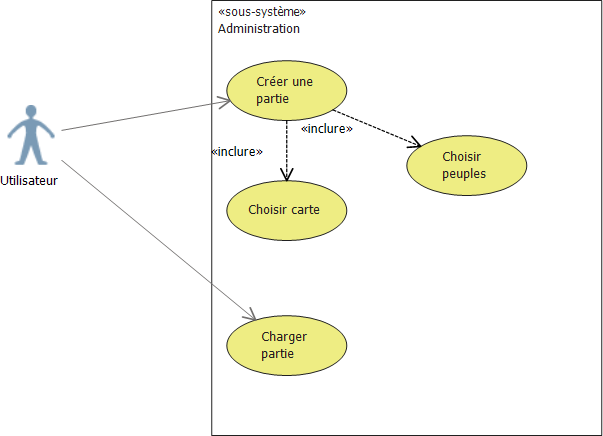
\includegraphics[width=\textwidth]{fig/diagramme_cas_utilisation_administration}
	\caption{Diagramme de cas d'utilisation : Adminisatration d'une partie}
	\label{dcu:ap}
\end{figure} 

\subsubsection{Diagramme de séquence}
Lors de la création d'une partie :
\begin{itemize}
\item On met en place les éléments de la partie. Pour cela,
	\begin{itemize}
	\item[$\bullet$] On utilise le patron de conception monteur.
	\item[$\bullet$] La classe \textbf{DirecteurPartie} fait appel la méthode  \textbf{creerJoueurs(carte, p1, p2)} de la classe \textbf{MonteurNvllePartie} si c'est une nouvelle partie et \textbf{MonteurChPartie} si c'est l'on charge une partie.
	\end{itemize}
\item On crée le peuple d'un joueur,
	\begin{itemize}
	\item[$\bullet$] La méthode \textbf{creerJoueur(carte,p1,p2)} va faire appel à une nouvelle instance de la fabrique \textbf{FabriquePeuple}.
	\item[$\bullet$] La fabrique va se charger de créer le bon nombre d'unité puis va retourner une instance de peuple (\textbf{Elf}, \textbf{Orc} ou \textbf{Nain}) qui possédera la liste des unités créées.
	\end{itemize}
\item On crée un joueur et on lui associe son peuple, 
	\begin{itemize}
	\item[$\bullet$] La méthode \textbf{creerJoueurs(carte,p1,p2)} va faire appel au constructeur de \textbf{Joueur} en lui passant le peuple qui lui sera attribué.
	\end{itemize}
\item On récupère la liste des joueurs et on la stocke dans la propriété \textit{joueurs}.
\item On crée la carte,
	\begin{itemize}
	\item[$\bullet$] Le monteur de partie va d'abord définir quel type (classe) de carte va être créé.
	\item[$\bullet$]  Ensuite, on crée la carte avec \textbf{creerCarte()}.
	\end{itemize}
\item On crée les cases de la carte,
	\begin{itemize}
	\item[$\bullet$] On utilise le patron de conception \textbf{poids-mouche} pour modéliser la classe.
	\item[$\bullet$] La carte (normale, petite, demo) va alors faire \textit{n} appels (n en fonction du type de carte) à la méthode \textbf{getCase(type)}. Cela va permettre de retourner une instance de la classe de case (désert, forêt, montagne, plaine) correspondant au type passé en paramètre, sachant qu'on a utilisé la \textit{lazy instanciation} pour l'instanciation des cases.
	\item[$\bullet$] On fait appel au constructeur de \textit{Carte} en lui passant la liste des cases créées en paramètre.
	\end{itemize}
\item On récupère ensuite la carte et on la stocke dans la propriété \textit{carte}.
\item On retourne ensuite l'instance de la partie qui vient d'être créée ou chargée. 
\item On se place dans l'attente d'un premier évènement.
\end{itemize}
\medskip
La figure \ref{ds:cp} représente le diagramme de séquence associé au scénario ci-dessus.
\begin{figure}[H]
	\centering
	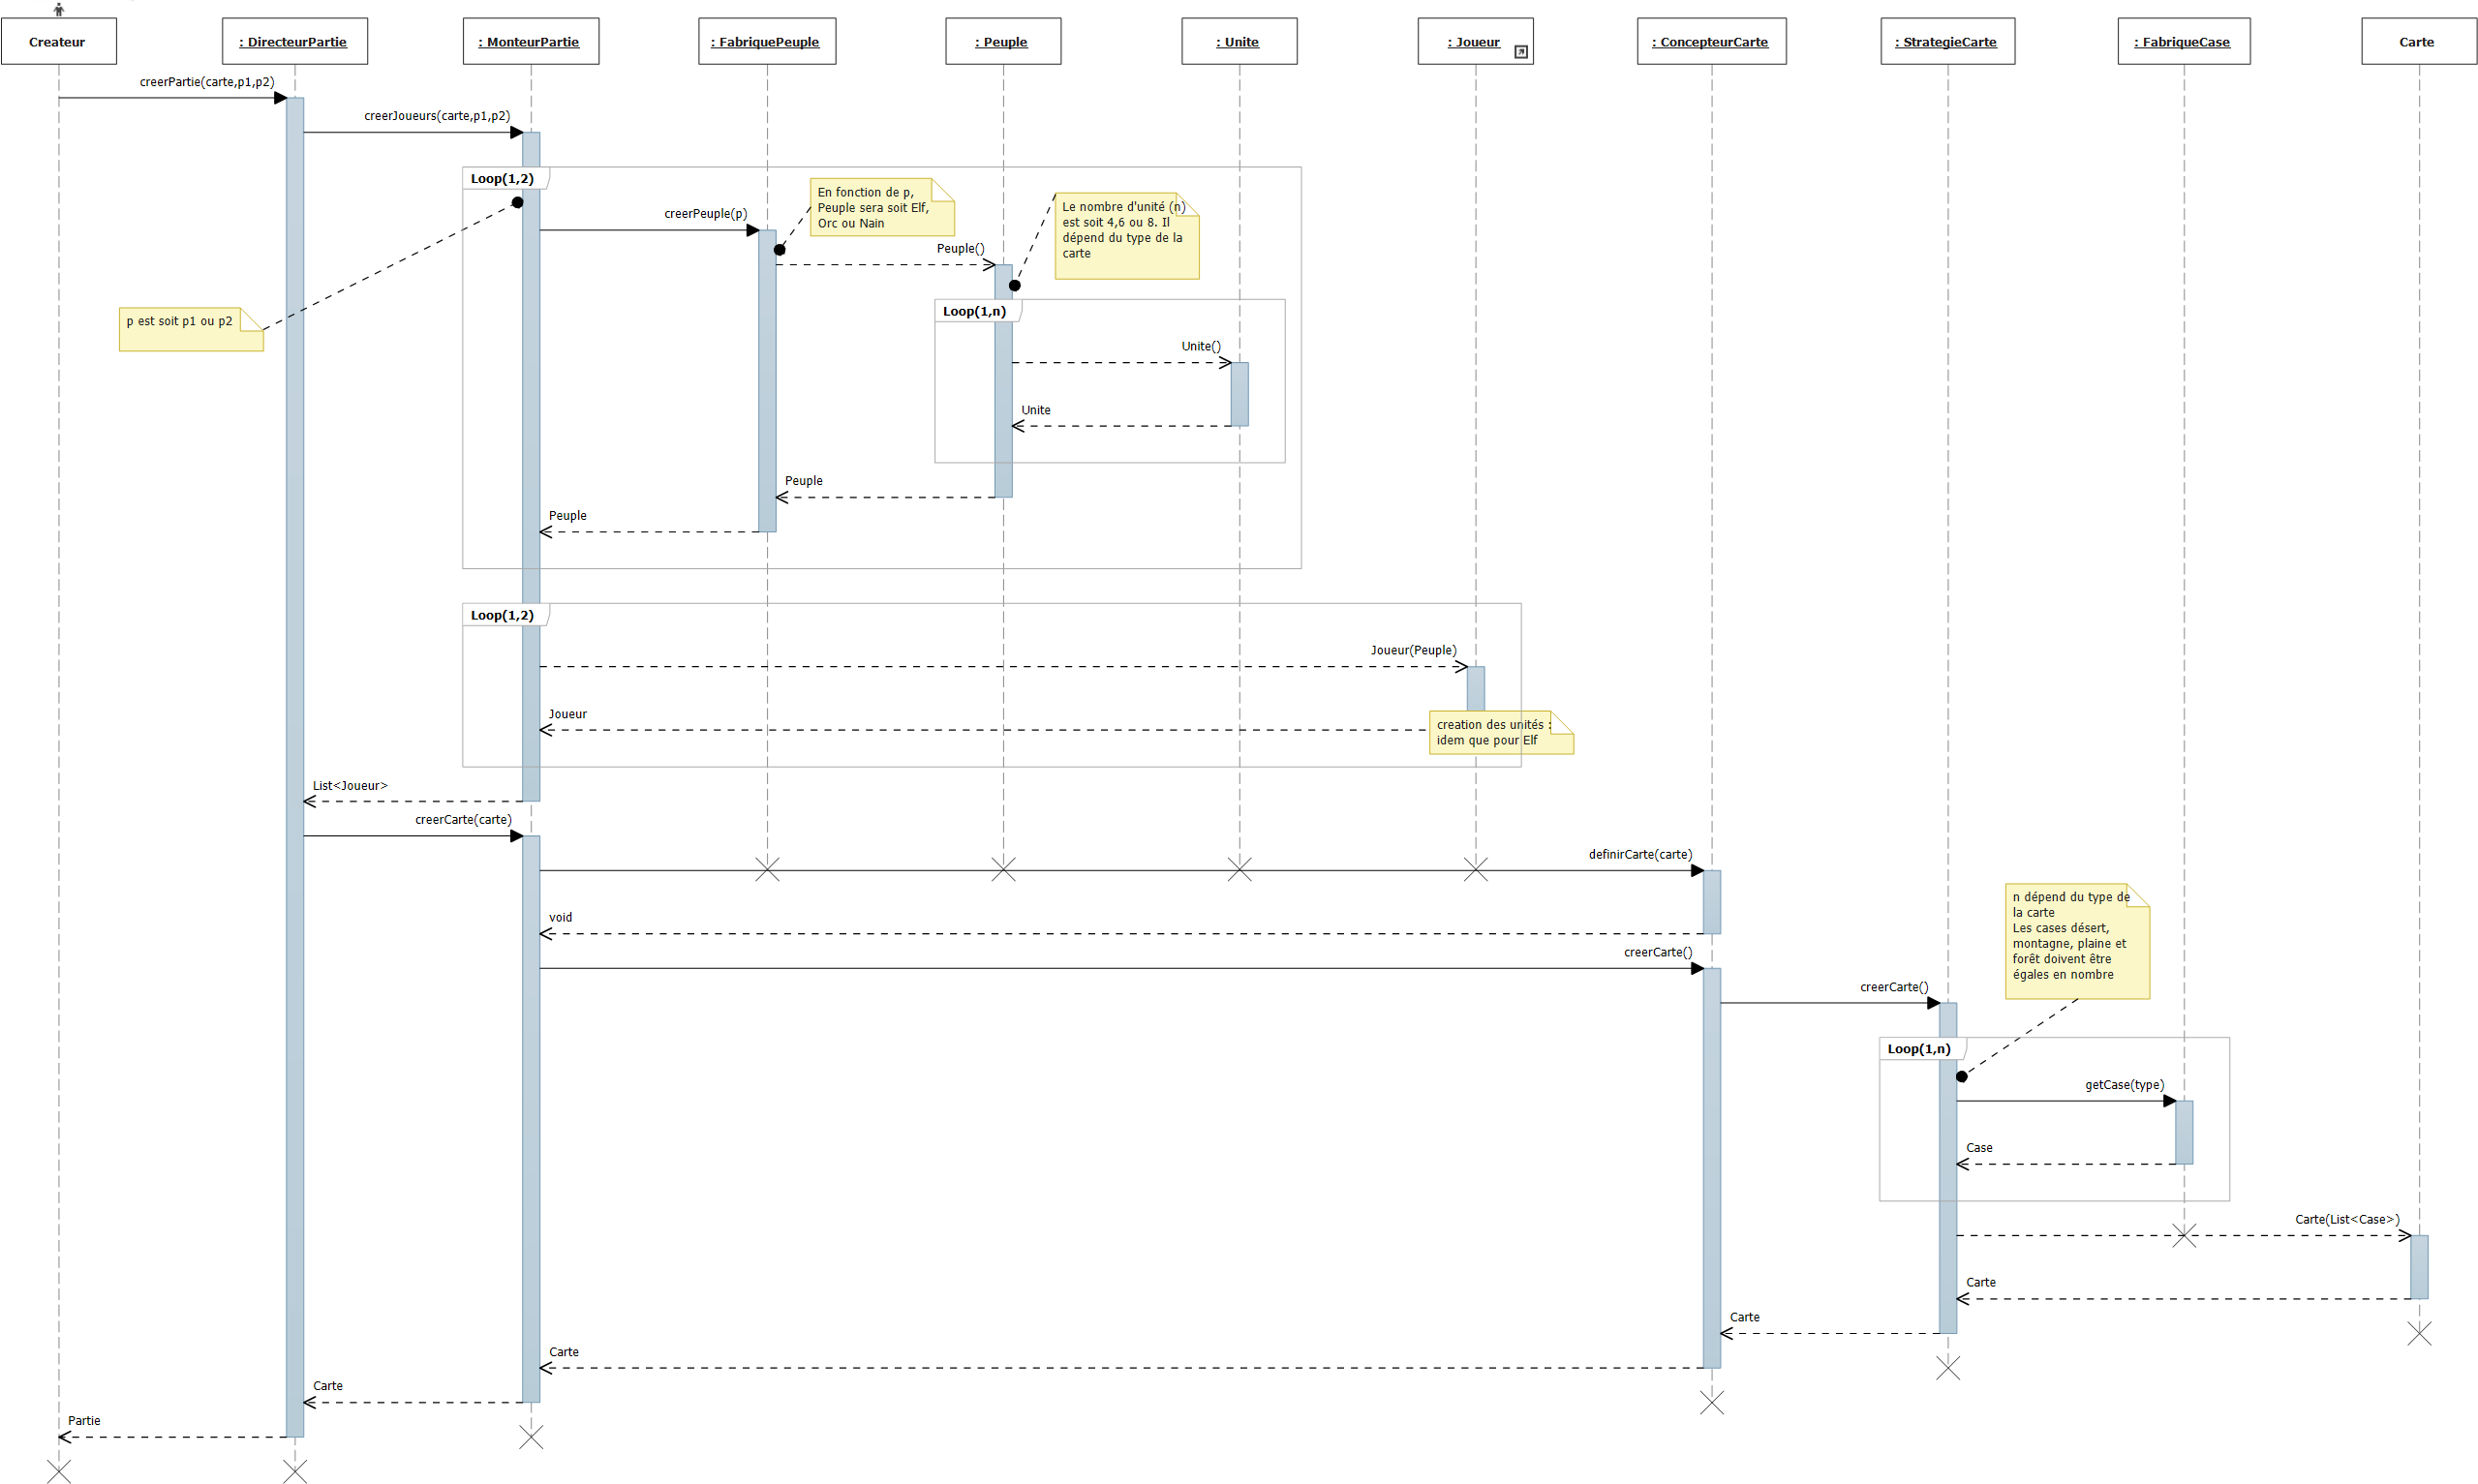
\includegraphics[width=\textwidth]{fig/diagramme_sequence_creerPartie}
	\caption{Diagramme de séquence : Création d'une partie}
	\label{ds:cp}
\end{figure} 
\subsection{Jouer une partie}
Lors d'une partie, les joueurs vont jouer alternativement. Le joueur peut afficher des informations sur une case ou une unité en cliquant gauche dessus. Il peut sélectionner une unité en faisant un clic gauche dessus, puis la déplacer en faisant clic droit sur la case. Si le joueur appuie sur espace, l'unité suivante est alors sélectionnée. \\
Le joueur peut aussi décider d'enregistrer la partie, la quitter ou déclarer forfait.\\
En supplément, le joueur peut décider d'afficher l'historique des coups joués.
\subsubsection{Diagramme de cas d'utilisation}
Le diagramme de cas d'utilisation associé à une partie est le suivant (Figure \ref{dcu:jp}). 
\begin{figure}[H]
	\centering
	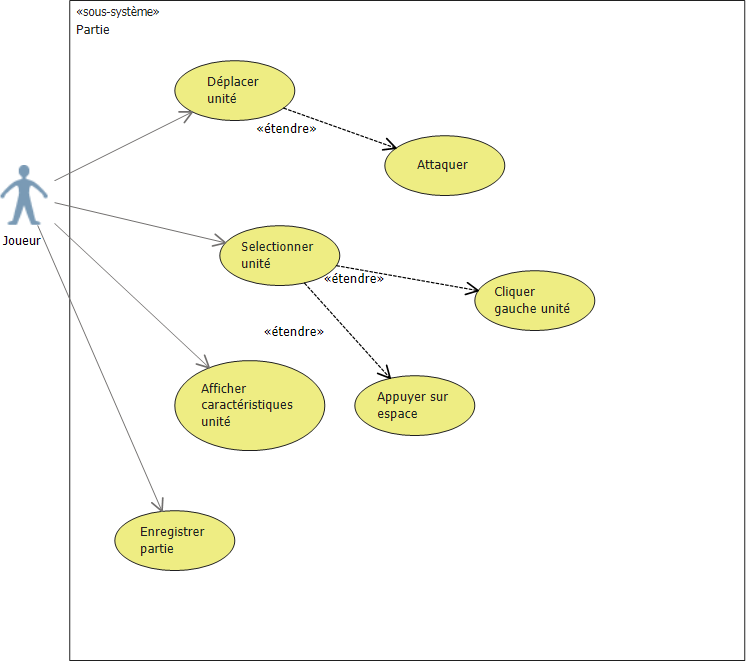
\includegraphics[width=\textwidth]{fig/diagramme_cas_utilisation_partie}
	\caption{Diagramme de cas d'utilisation : Jouer une partie}
	\label{dcu:jp}
\end{figure} 
\subsubsection{Diagramme de séquence}
Lorsque la partie est lancée, celle-ci se met en attente d'événement qui va déclencher certains algorithmes.
\begin{itemize}
\item L'utilisateur peut cliquer sur une case.
	\begin{itemize}
	\item[$\bullet$] On met à jour le x et le y de la partie pour les faire correspondre à la case.
	\item[$\bullet$] Ensuite, soit une unité n'est pas sélectionnée,
		\begin{itemize}
		\item[-] On vérifie si la case se compose d'une unité du joueur. Si oui, on retourne la liste des unités sur la case. Sinon, on retourne null.
		\item[-] S'il y a plusieurs unités dans la liste, on demande à l'utilisateur de choisir celle qu'il souhaite utiliser.
		\item[-] Dès que l'unité est choisie, on modifie la valeur de la propriété uniteCourante.
		\end{itemize}
	\item[$\bullet$] Soit une unité est sélectionnée,
		\begin{itemize}
		\item[-] On lance l'action de déplacer l'unité sur la case. 
		\item[-] Une fois l'action terminée, on vérifie s'il reste des unités de chaque côté. Auquel cas, on continue la partie sinon on déclare le vainqueur.
		\end{itemize}
	\end{itemize}
\item L'utilisateur fini son tour.
	\begin{itemize}
	\item[$\bullet$] On calcule son nombre de points
	\item[$\bullet$] On vérifie que le nombre de tour max n'est pas atteint auquel cas on regarde quel joueur à le plus point et on déclare le vainqueur.
	\item[$\bullet$] On passe la main au joueur suivant.
	\end{itemize}
\end{itemize}
La figure \ref{ds:jp} représente le diagramme de séquence associé au scénario ci-dessus.
\begin{figure}[H]
	\centering
	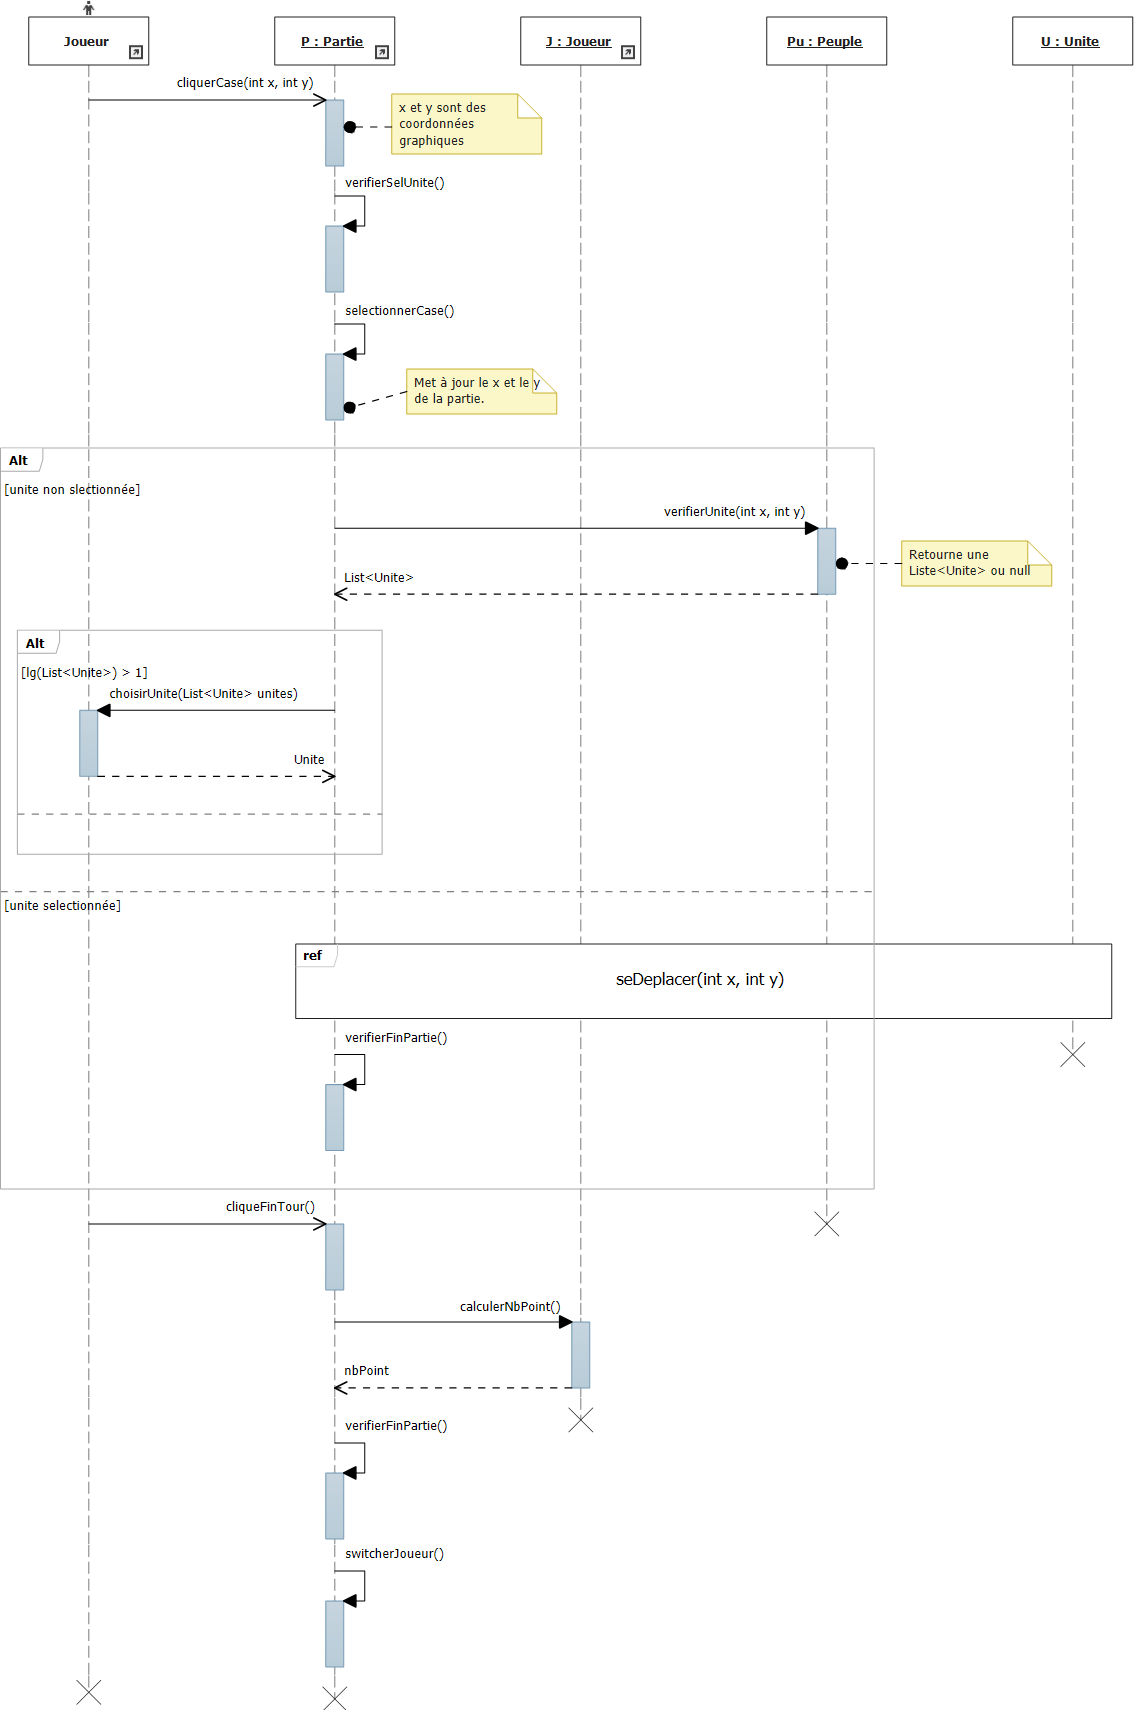
\includegraphics[width=\textwidth]{fig/diagramme_sequence_jouerTour}
	\caption{Diagramme de séquence : Jouer une partie}
	\label{ds:jp}
\end{figure} 
\subsubsection{Etat d'une unité}
Les unités sur la carte possèdent deux groupes d'états ; en sélection et en activité. Lorsqu'une unité est en sélection, elle peut être dans deux états. Soit elle en attente, c'est-à-dire non sélectionnée, soit elle est active, c'est-à-dire sélectionnée. Lorsqu'une unité est sélectionnée, elle est mise en surbrillance. Une unité peut être sélectionnée par un clic ou bien par la pression de la barre d'espace si c'est à son tour. Si une unité est sélectionnée, elle est desélectionnée si on fait un clic gauche sur une autre case ou que l'on fait espace.\\
Dans le groupe d'état en activité, il y a deux états. Soit elle est en déplacement, c'est-à-dire que l'unité se déplace sur une autre case, soit elle est en combat contre une unité adverse. 
Une unité passe de l'état sélectionné à en activité si le joueur fait un clic droit sur une autre case. Si celle-ci possède des unités adverses, alors l'unité passe en état de combat, sinon elle passe en état de déplacement. A la fin de l'état combat, si l'unité a perdu, on vérifie ses points de vie. S'ils sont supérieurs à zéro, l'unité repasse en état de sélection active. Sinon, l'unité est détruite.\\
En revanche, si l'unité gagne le combat, on vérifie s'il reste des unités adverses sur la case. Si oui, on repasse l'unité en état de sélection active. Sinon, on la fait passer en état de déplacement puis en état de sélection active. 
\begin{figure}[H]
	\centering
	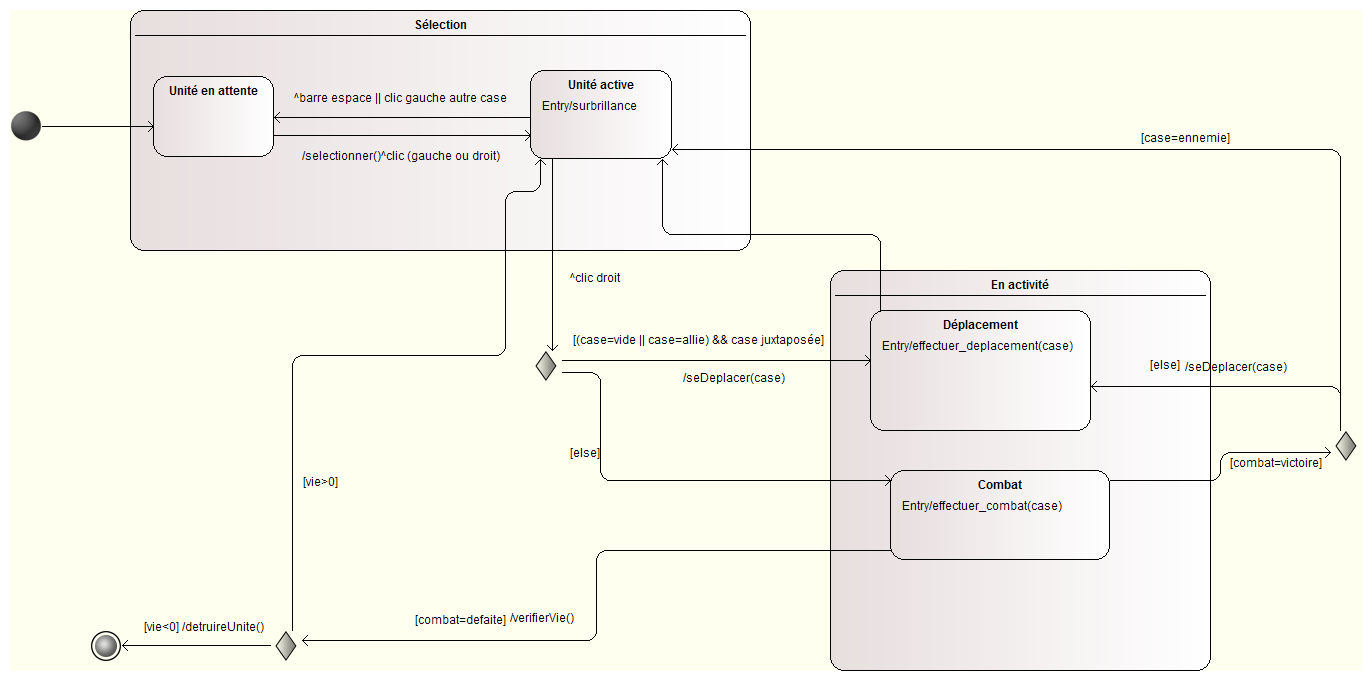
\includegraphics[width=\textwidth]{fig/diagramme_etat_transition_unite_modelio}
	\caption{Diagramme d'états de transition : Unité}
	\label{det:e}
\end{figure} 
\subsubsection{Se déplacer}
Lorsqu'une unité est sélectionnée par le joueur, il peut choisir de la déplacer sur une case juxtaposée. Pour ce faire, l'utilisateur clique (clic droit) sur une case. Si l'unité ne possède pas assez de points de déplacement pour aller sur cette case (bonus de déplacement compris), un message d'erreur s'affiche. Sinon, on vérifie qu'aucune unité adverse n'est présente sur cette. Si tel est le cas, on lance le scénario de combat (partie \ref{subsub:cbt}). Sinon, on déplace l'unité sur la case.\\
Afin de modéliser un déplacement, on a conçu un diagramme d'activité (Figure \ref{da:dep}).
\begin{figure}[H]
	\centering
	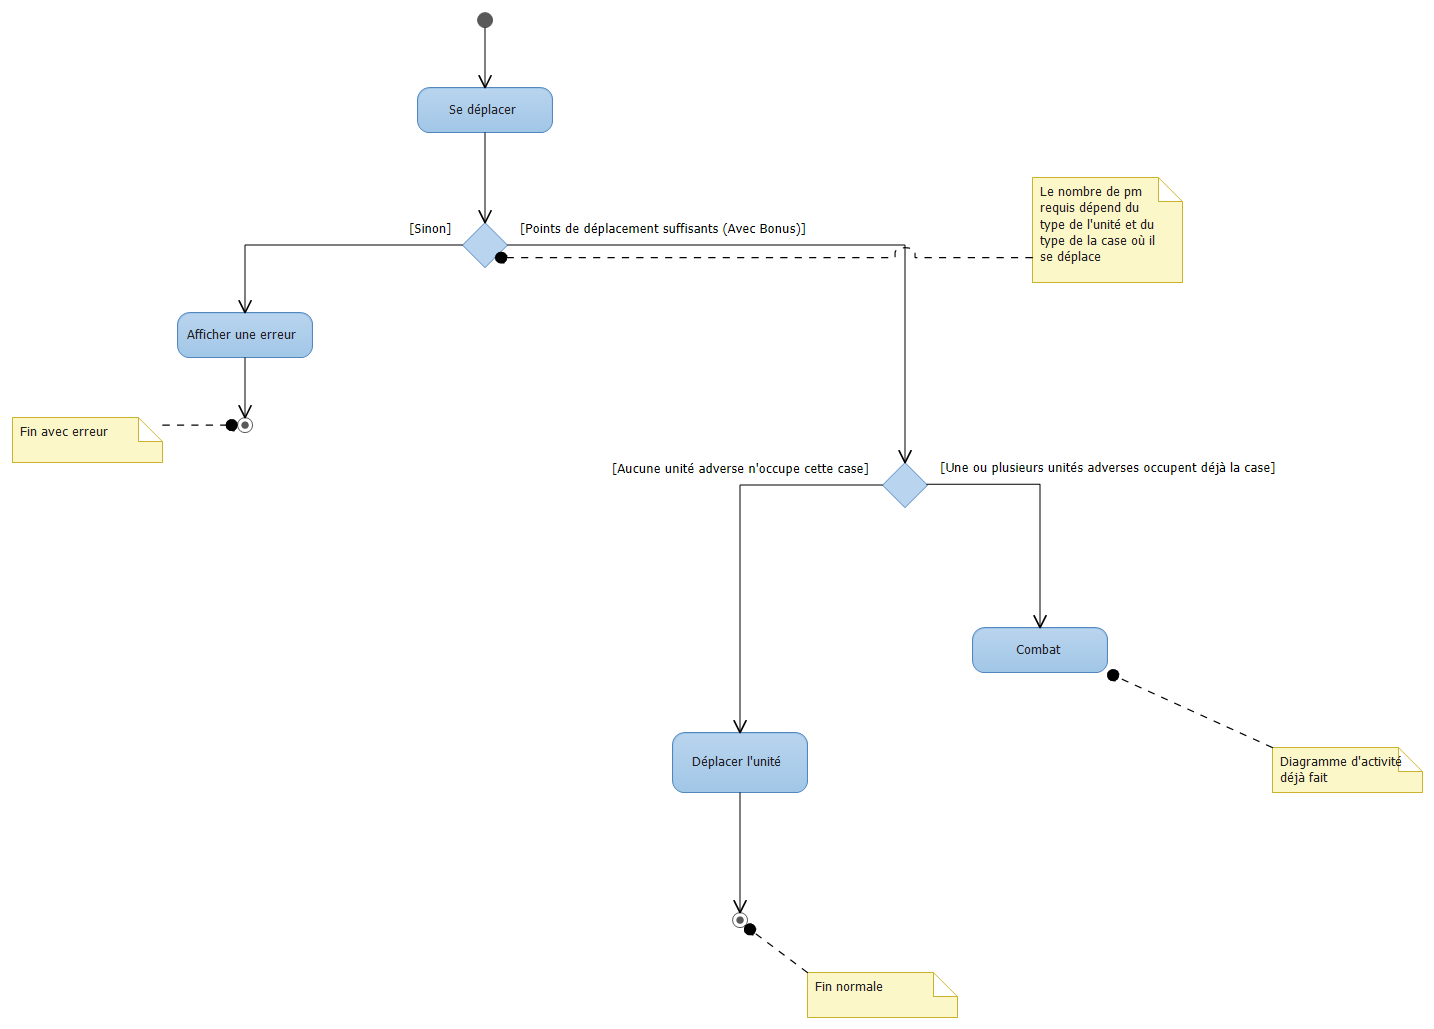
\includegraphics[width=\textwidth]{fig/diagramme_activite_deplacerUnite}
	\caption{Diagramme d'activité : Déplacement}
	\label{da:dep}
\end{figure}   
\subsubsection{Combattre}
Le combat débute lorsqu'une unité se déplace sur une case où se situe une unité adverse. La première chose à faire est de vérifier le nombre d'unités adverses situées sur la case. S'il y a plus d'une unité sur la case, il faut alors choisir l'unité possédant les meilleurs caractéristiques de défense (vie et point de défense). La meilleure unité est choisie pour le combat. S'il y a égalité entre les unités défensives, l'une d'entre-elles est choisie aléatoirement.\\ 
\label{subsub:cbt}
Une fois que les deux unités ont été sélectionnées pour effectuer le combat, on procède au calcul du nombre de combat. On calcule aussi la probabilité de chance de victoire pour l'unité offensive et défensive. L'attaque se produit. Si l'attaque réussie, l'unité défensive perd un point de vie. Dans le cas contraire, c'est l'unité offensive qui perd un point de vie.\\ 
On vérifie ensuite si l'une des unités est morte (0 point de vie). Si l'unité offensive est morte, on quitte le combat et on retourne à l'action de déplacement en signalant la \textit{défaite}. Si l'unité défensive meurt, on déplace l'unité offensive si aucune autre unité adverse n'occupe encore la case. Dans ce cas, on retourne \textit{victoire}. Si à la fin des combats aucune des deux unités n'est morte, on retourne \textit{nul}.\\
Le diagramme d'activité correspondant à l'action \textbf{combattre} est le suivant (Figure \ref{da:cbt}):
\begin{figure}[H]
	\centering
	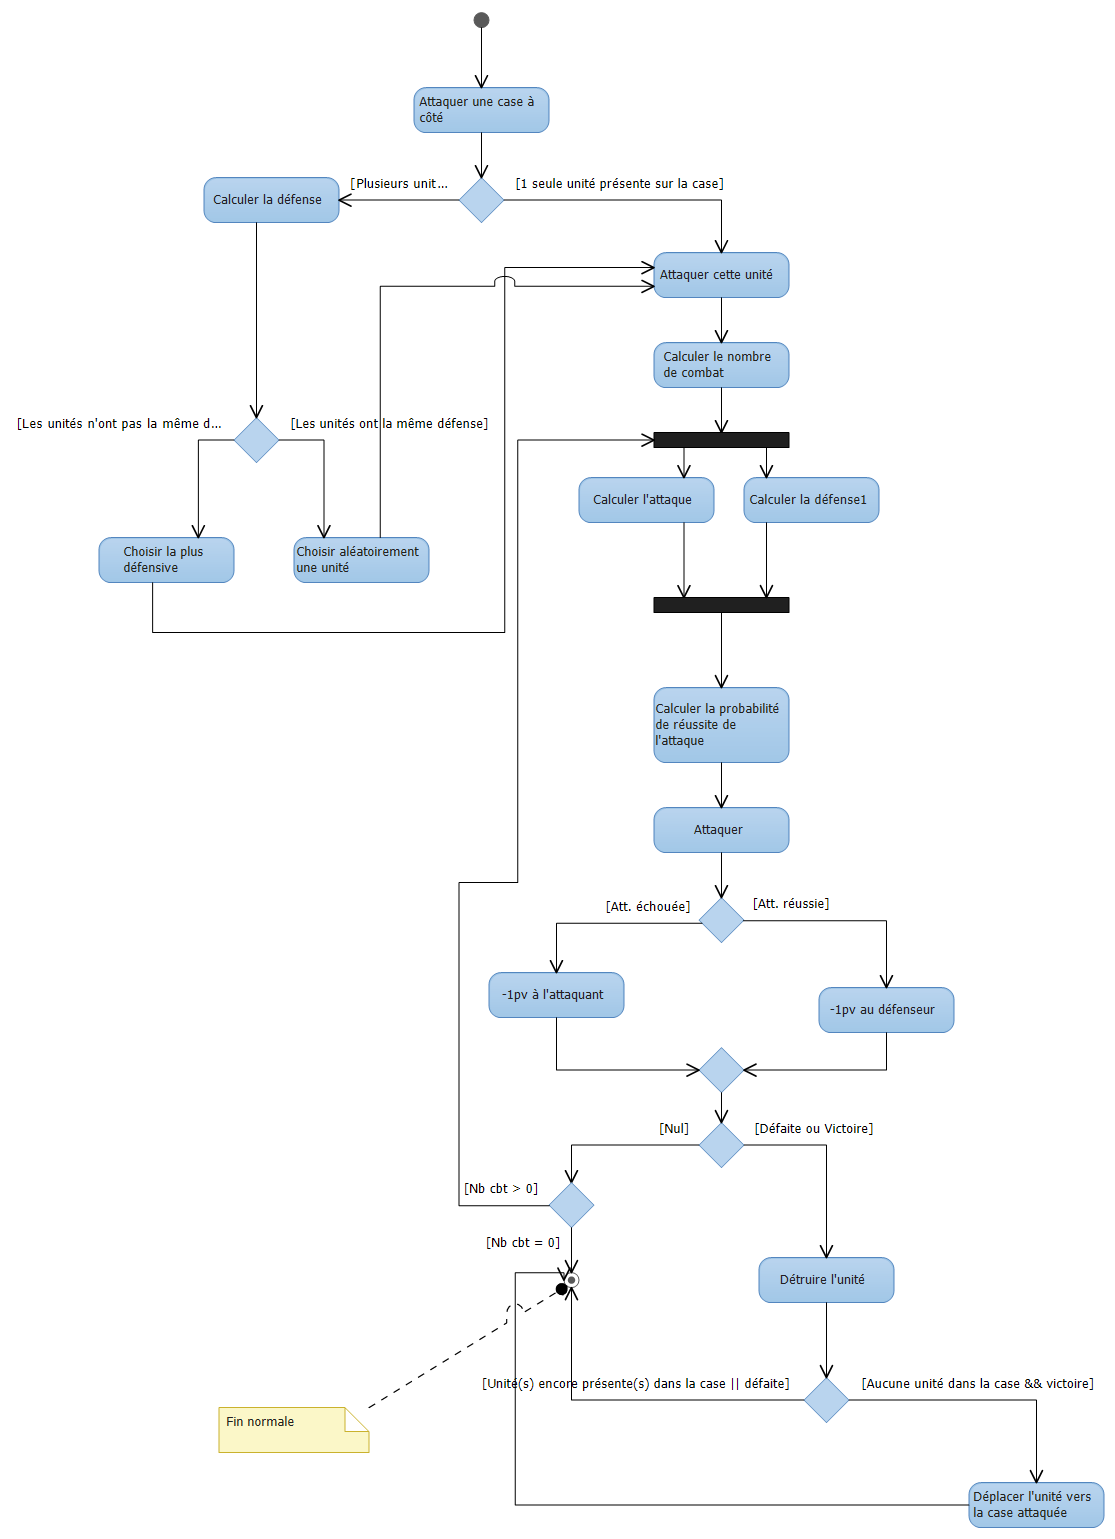
\includegraphics[width=\textwidth]{fig/diagramme_activite_combatUnite}
	\caption{Diagramme d'activité : Combat}
	\label{da:cbt}
\end{figure}

\subsection{Synthèse}
%intro diagramme de classe
Les diagrammes de cas d'utilisation, d'interaction et d'états de transition nous ont permis de représenter des cas d'usage de notre jeu et de les expliquer étape par étape en explicitant les noms des méthodes. Dans cette partie, nous allons présenter notre modèle de classe, ainsi que les patrons de conception qui ont été utilisés.
\subsubsection{Patrons de conception}
\paragraph{Monteur}\mbox{}\medskip\\
Ce patron a été utilisé afin de créer une nouvelle partie ou bien d'en charger une qui est déjà enregistrée. Son but est de ne pas allourdir la classe partie, puisque la création d'un tel objet \textbf{Partie} est complexe. La figure \ref{pc:mp} montre le modèle monteur utilisé.
\begin{figure}[H]
	\centering
	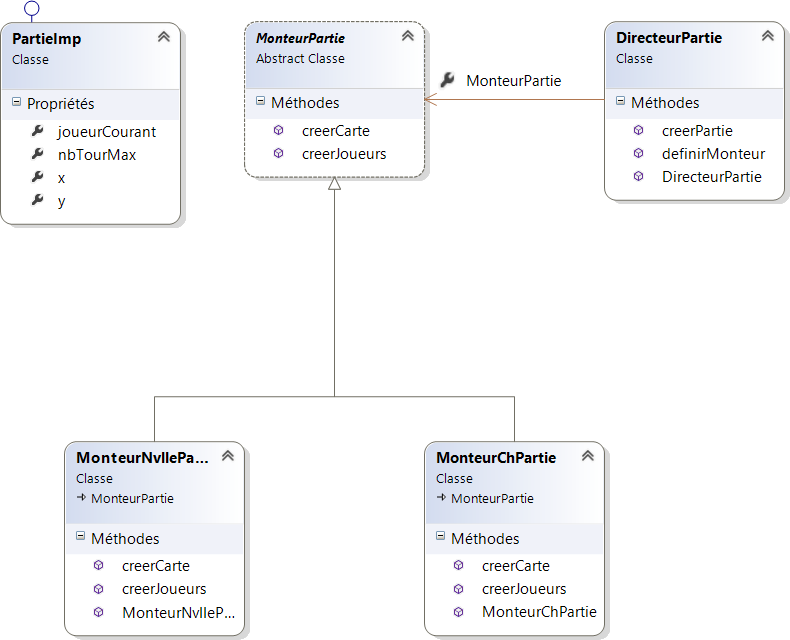
\includegraphics[width=\textwidth]{fig/monteur_partie}
	\caption{Patron de conception : Monteur Partie}
	\label{pc:mp}
\end{figure}

\paragraph{Stratégie}\mbox{}\medskip\\
Le patron \textbf{Stratégie} permet de créer différents types de carte en passant en paramètre l'instance de la carte (demo, petite, normale) lors de la définition de celle-ci. Il permet également de changer le type de la carte en cours de partie.
\begin{figure}[H]
	\centering
	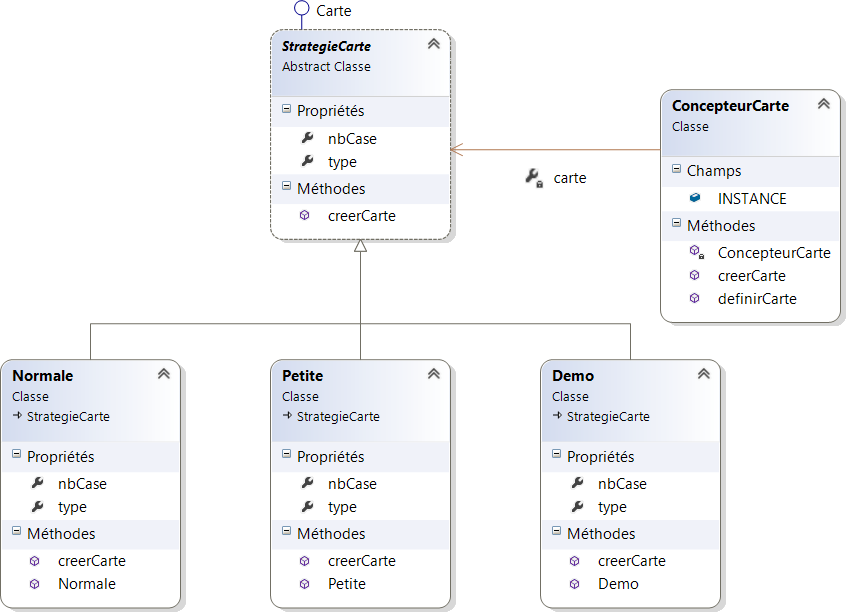
\includegraphics[width=\textwidth]{fig/strategie_carte}
	\caption{Patron de conception : Stratégie Carte}
	\label{pc:sc}
\end{figure}

\paragraph{Poids-Mouche}\mbox{}\medskip\\
Afin de limiter l'instanciation des classes cases (montagne, forêt, deset, plaine), nous avons utilisé le patron \textbf{Poids-Mouche}. En effet, lors de la création de la carte, la stratégie fait appel à \textbf{getCase} en passant comme paramètre le type de la case à créer. Cette dernière retourne la case attendue après l'avoir créée si cette dernière n'est pas déjà instanciée. Cette méthode s'appelle \textit{Lazy Instanciation}.
\begin{figure}[H]
	\centering
	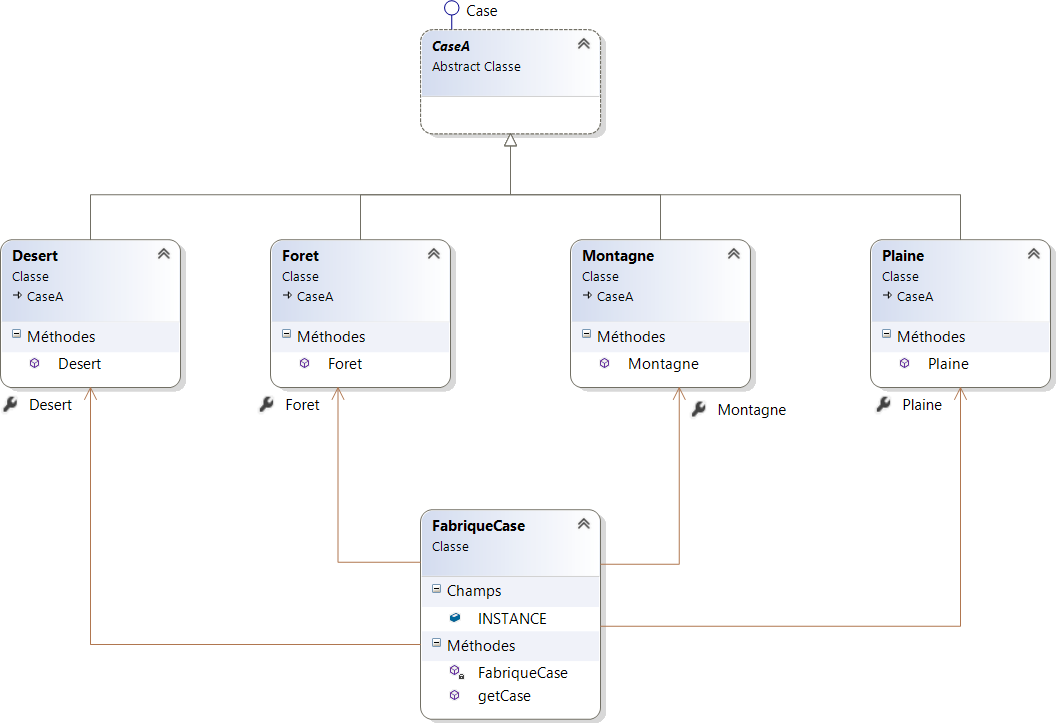
\includegraphics[width=\textwidth]{fig/poidsmouche_case}
	\caption{Patron de conception : Poids-Mouche Case}
	\label{pc:pmc}
\end{figure}

\paragraph{Fabrique}\mbox{}\medskip\\
Le patron \textbf{Fabrique} gère la création des peuples (Orc, Elf, Nain). Il a été utilisé afin de manipuler les interfaces et non pas les types concrets, ainsi que de factoriser la création des peuples dans une seule classe.
\begin{figure}[H]
	\centering
	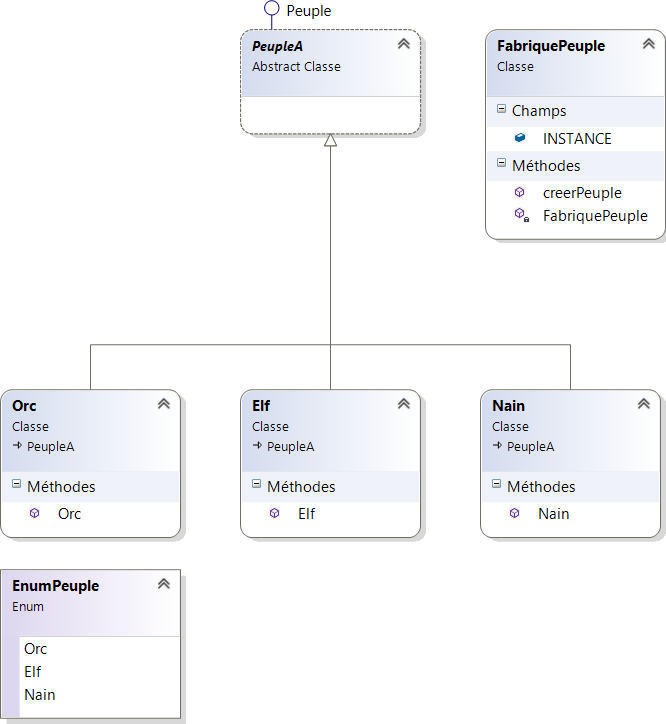
\includegraphics[width=\textwidth]{fig/fabrique_peuple}
	\caption{Patron de conception : Fabrique peuple}
	\label{pc:fp}
\end{figure}

\subsubsection{Diagramme de classe}
\begin{figure}[H]
	\centering
	\rotatebox{90}{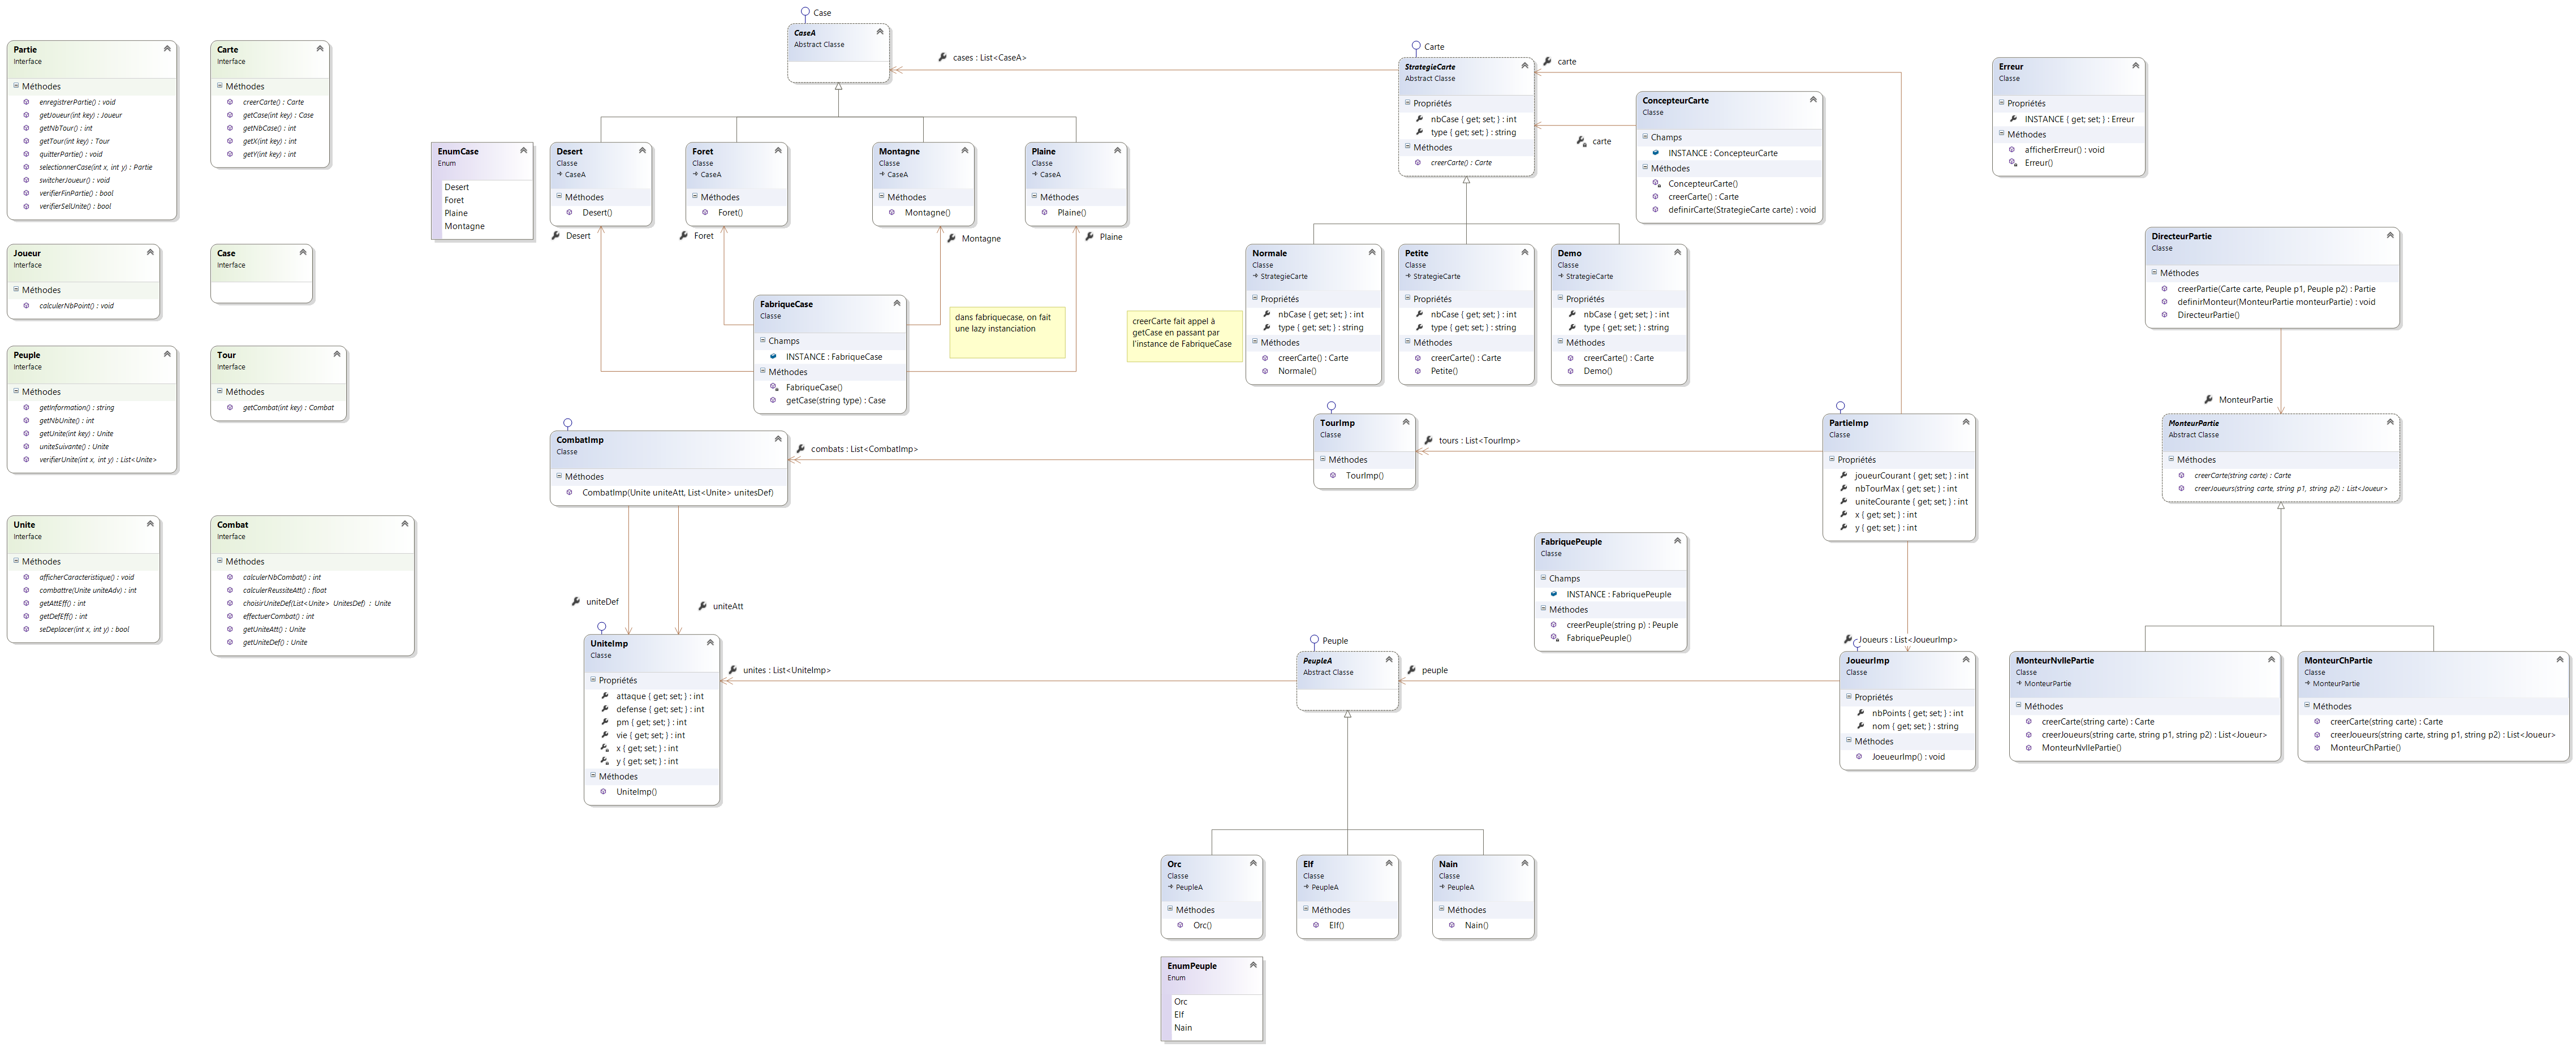
\includegraphics[width=\paperwidth]{fig/diagramme_de_classe}}
	\caption{Diagramme de classe}
	\label{dc}
\end{figure}

\section{Conclusion}
Nous venons de réaliser la partie conception du projet. Cela nous a permis de bien appréhender la partie modèle. Grâce à cela, nous allons certainement gagner du temps lors de la réalisation du projet puisque nous possédons une bonne vision de ce que nous avons à réaliser. De plus, le gain de temps se réalise de façon concrète puisque le diagramme de classes va nous permettre de générer les classes avec leurs attributs et méthodes.\medskip\\
Nous allons maintenant devoir réaliser l'implémentation du modèle et la partie graphique du projet. Pour cela, nous nous sommes mis à disposition un GIT qui nous permettra de tenir à jour l'avancement de notre projet.\medskip\\
Dans un premier temps, nous avons pour objectif de réaliser les tâches qui nous sont demandées. Une fois que toutes ces tâches auront été accomplies, nous allons alors créer une première version du jeu qui sera jouable.\medskip\\
Ensuite, s'il nous reste du temps, nous réaliserons des tâches annexes qui nous sont proposées ou que nous souhaitons mettre en place. Cela nous permettra de produire une seconde version.\medskip\\
Si cela est possible, nous souhaitons aussi créer une version plus évoluée du jeu au niveau des combats et du déplacement sur la carte. On peut aussi ajouter de nouveaux objectifs comme des objets ou des actions à réaliser qui permettront d'obtenir des bonus. Cette version ne sera pas remise pour examen sauf si nous recevons une indication contraire. Mais ici encore, cette version ne sera développée uniquement si nous avons le temps.\medskip\\
Lors de ce projet, nous devons réaliser des tests de conception. Les versions finales de ce projet seront des applications WPF.
\newpage
\listoffigures
\end{document}